% File: thesis/figures/fig_3_17_lhs_vs_random.tex
\documentclass[tikz,border=10pt]{standalone}
\usepackage{tikz}
\usepackage{amsmath}
\usepackage{amssymb}
\usepackage{pgfplots}
\pgfplotsset{compat=1.18}
\usetikzlibrary{
    arrows.meta, 
    positioning, 
    calc,
    patterns,
    fit,
    backgrounds
}

% Colors
\definecolor{lhsblue}{RGB}{66,133,244}         % LHS points
\definecolor{randomred}{RGB}{234,67,53}        % Random points
\definecolor{cormap}{RGB}{162,59,114}          % Correlation color
\definecolor{gridgray}{RGB}{189,189,189}       % Grid lines

\begin{document}
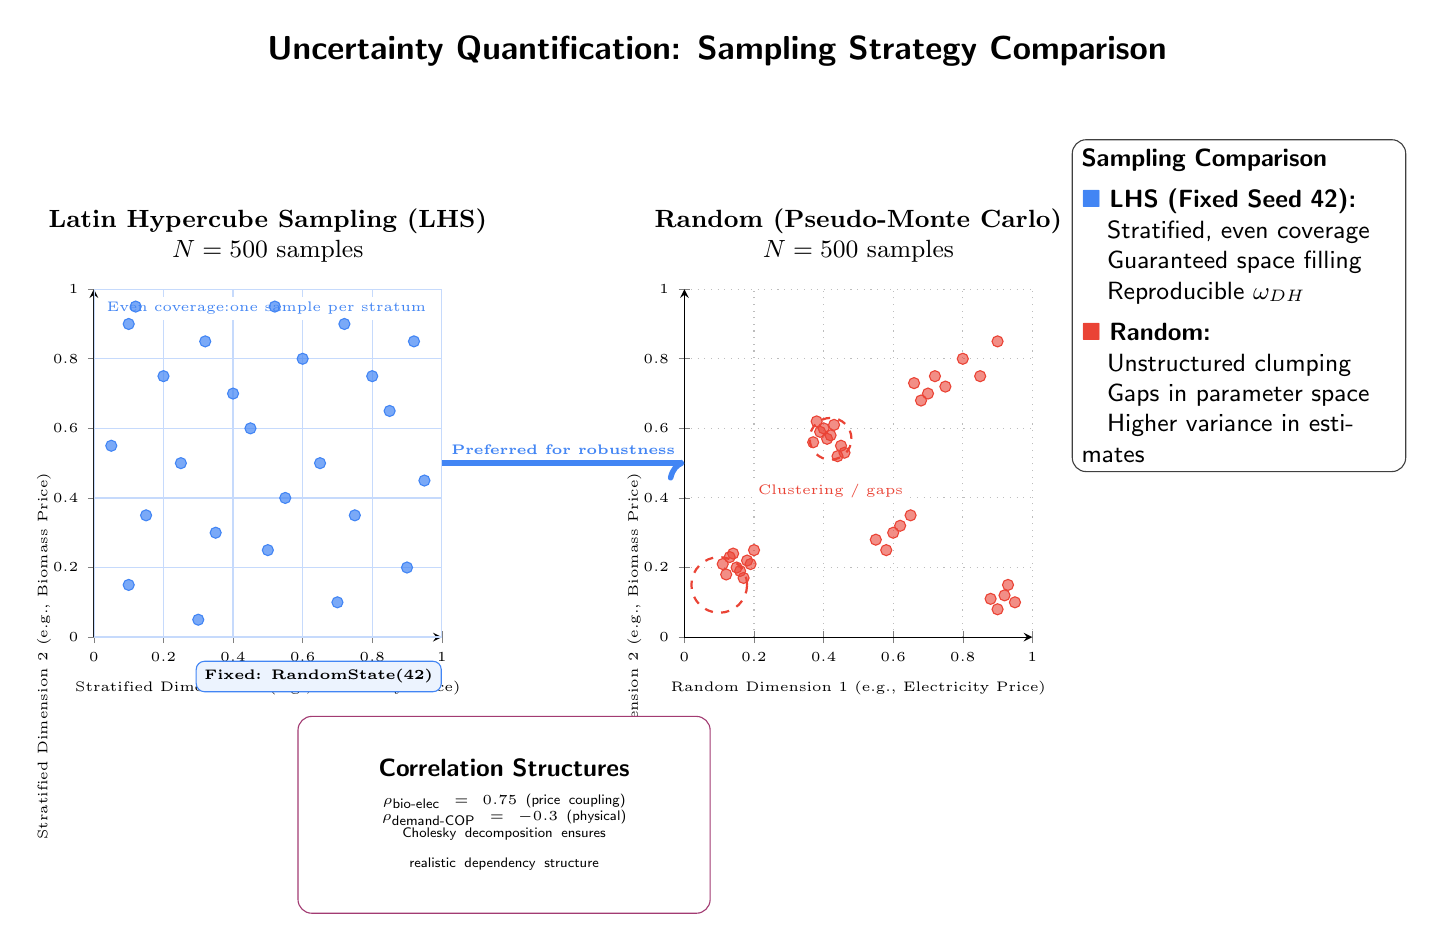
\begin{tikzpicture}[
    font=\small\sffamily
]

% === LEFT PLOT: LATIN HYPERCUBE SAMPLING ===
\begin{axis}[
    name=lhsplot,
    at={(0,0)},
    anchor=south west,
    width=6cm,
    height=6cm,
    xtick={0,0.2,0.4,0.6,0.8,1},
    ytick={0,0.2,0.4,0.6,0.8,1},
    xmin=0, xmax=1,
    ymin=0, ymax=1,
    xlabel={Stratified Dimension 1 (e.g., Electricity Price)},
    ylabel={Stratified Dimension 2 (e.g., Biomass Price)},
    xlabel style={font=\tiny, below},
    ylabel style={font=\tiny, left},
    tick label style={font=\tiny},
    title={\textbf{Latin Hypercube Sampling (LHS)}\\$N=500$ samples},
    title style={font=\small, align=center},
    axis lines=left,
    grid=major,
    grid style={gridgray, dotted},
]

% Draw stratification grid (5x5 for visualization, conceptually 500)
\pgfplotsinvokeforeach{0,0.2,0.4,0.6,0.8,1} {
    \draw[lhsblue!30, line width=0.5pt] (axis cs:#1,0) -- (axis cs:#1,1);
    \draw[lhsblue!30, line width=0.5pt] (axis cs:0,#1) -- (axis cs:1,#1);
}

% LHS points (evenly distributed - one per stratum)
% Simulating 25 visible points for clarity (representing 500)
\addplot[
    only marks,
    mark=*,
    mark size=2pt,
    lhsblue,
    fill opacity=0.7
] coordinates {
    (0.1,0.15) (0.3,0.05) (0.5,0.25) (0.7,0.1) (0.9,0.2)
    (0.15,0.35) (0.35,0.3) (0.55,0.4) (0.75,0.35) (0.95,0.45)
    (0.05,0.55) (0.25,0.5) (0.45,0.6) (0.65,0.5) (0.85,0.65)
    (0.2,0.75) (0.4,0.7) (0.6,0.8) (0.8,0.75) (0.1,0.9)
    (0.12,0.95) (0.32,0.85) (0.52,0.95) (0.72,0.9) (0.92,0.85)
};

% Label for even coverage
\node[anchor=north west, font=\tiny, lhsblue, fill=white, inner sep=2pt] 
    at (axis cs:0.02,0.98) {Even coverage:\\one sample per stratum};

\end{axis}

% === RIGHT PLOT: RANDOM SAMPLING ===
\begin{axis}[
    name=randplot,
    at={(7.5cm,0)},
    anchor=south west,
    width=6cm,
    height=6cm,
    xtick={0,0.2,0.4,0.6,0.8,1},
    ytick={0,0.2,0.4,0.6,0.8,1},
    xmin=0, xmax=1,
    ymin=0, ymax=1,
    xlabel={Random Dimension 1 (e.g., Electricity Price)},
    ylabel={Random Dimension 2 (e.g., Biomass Price)},
    xlabel style={font=\tiny, below},
    ylabel style={font=\tiny, left},
    tick label style={font=\tiny},
    title={\textbf{Random (Pseudo-Monte Carlo)}\\$N=500$ samples},
    title style={font=\small, align=center},
    axis lines=left,
    grid=major,
    grid style={gridgray, dotted},
]

% Random points (clumped distribution)
\addplot[
    only marks,
    mark=*,
    mark size=2pt,
    randomred,
    fill opacity=0.6
] coordinates {
    % Cluster 1 (clumping)
    (0.15,0.2) (0.18,0.22) (0.12,0.18) (0.2,0.25) (0.14,0.24)
    (0.16,0.19) (0.19,0.21) (0.13,0.23) (0.17,0.17) (0.11,0.21)
    % Sparse area
    (0.8,0.8) (0.85,0.75) (0.9,0.85)
    % Cluster 2
    (0.4,0.6) (0.45,0.55) (0.42,0.58) (0.38,0.62) (0.44,0.52)
    (0.41,0.57) (0.46,0.53) (0.39,0.59) (0.43,0.61) (0.37,0.56)
    % More scattered points
    (0.6,0.3) (0.65,0.35) (0.55,0.28) (0.62,0.32) (0.58,0.25)
    (0.7,0.7) (0.75,0.72) (0.68,0.68) (0.72,0.75) (0.66,0.73)
    % Edge cluster
    (0.95,0.1) (0.92,0.12) (0.9,0.08) (0.93,0.15) (0.88,0.11)
};

% Show clumping problem
\draw[randomred, thick, dashed] (axis cs:0.1,0.15) ellipse (0.08 and 0.08);
\draw[randomred, thick, dashed] (axis cs:0.42,0.57) ellipse (0.06 and 0.06);
\node[font=\tiny, randomred, fill=white, inner sep=2pt] 
    at (axis cs:0.42,0.42) {Clustering / gaps};

\end{axis}

% === CORRELATION STRUCTURE INSET (Bottom) ===
\node[
    rectangle,
    draw=cormap,
    fill=white,
    rounded corners=5pt,
    text width=5cm,
    minimum height=2.5cm,
    align=center,
    below=1cm of lhsplot.south,
    xshift=3cm
] (correlation) {%
    \textbf{Correlation Structures}\\[4pt]
    \tiny
    $\rho_{\text{bio-elec}} = 0.75$ (price coupling)\\
    $\rho_{\text{demand-COP}} = -0.3$ (physical)\\
    Cholesky decomposition ensures\\
    realistic dependency structure
};

% === LEGEND BOX ===
\node[
    rectangle,
    draw=darkgray,
    fill=white,
    rounded corners=5pt,
    text width=4cm,
    minimum height=2cm,
    align=left,
    right=0.5cm of randplot.east,
    yshift=2cm
] (legend) {%
    \textbf{Sampling Comparison}\\[4pt]
    \textcolor{lhsblue}{$\blacksquare$} \textbf{LHS (Fixed Seed 42):}\\
    \quad Stratified, even coverage\\
    \quad Guaranteed space filling\\
    \quad Reproducible $\omega_{DH}$\\[4pt]
    \textcolor{randomred}{$\blacksquare$} \textbf{Random:}\\
    \quad Unstructured clumping\\
    \quad Gaps in parameter space\\
    \quad Higher variance in estimates
};

% === FIXED SEED ANNOTATION ===
\node[
    rectangle,
    draw=lhsblue,
    fill=lhsblue!10,
    rounded corners=3pt,
    font=\tiny\bfseries,
    inner sep=3pt,
    below=0.3cm of lhsplot.south east,
    anchor=north east
] {Fixed: RandomState(42)};

% === TITLE ===
\node[above=0.8cm of current bounding box.north, font=\large\bfseries\sffamily] {%
    Uncertainty Quantification: Sampling Strategy Comparison%
};

% === ARROWS SHOWING BENEFIT ===
\draw[->, line width=2pt, lhsblue] (lhsplot.east) -- (randplot.west)
    node[midway, above, font=\tiny\bfseries, fill=white, inner sep=2pt] 
    {Preferred for robustness};

\end{tikzpicture}
\end{document}
